\chapter{绪论} 
\section{非线性偏微分方程精确解的研究背景与相关工作}
In recent years, nonlinear evolution equations (NLEEs) have attracted particular attention from mathematicians, physicists and engineers. There are varieties of methods to construct exact solutions of NLEEs, such as the Inverse Scattering Method \cite{kawata1978inverse,ma2014verifying}, Darboux transformation method \cite{matveev1991darboux,ling2018general,lou1997non}, B{\"a}cklund transformation method \cite{wahlquist1973backlund,li2008method,cheng2015multiple}, Hirota bilinear method \cite{hirota1971exact,hereman1991exact,hu2002application,hirota2003vector,ma2015lump} and Wronskian technique \cite{freeman1983soliton,ito1988reduce,wu2008n}, etc. By using such varieties of schemes, several kinds of exact solutions are obtained, such as solitons \cite{hirota1971exact,makhankov1980computer}, breathers \cite{tajiri1989breather,guo2011rogue,sun2018general}, lump solutions \cite{satsuma1979two,villarroel1999discrete,imai1997dromion}, rogue waves \cite{guo2011rogue,zhang2014rogue,sun2018general,zhaqilao2018symbolic}, and so on.

Hirota bilinear method \cite{hirota1971exact}, which was proposed in 1971, plays an important role in the solving of NLEEs. Especially, the Hirota method is usually applied to construct soliton solutions of NLEEs. With the obtained soliton solutions, we can further calculate breather and lump solutions by the conjugate parameter assignment \cite{tajiri1989breather} and long wave limit \cite{satsuma1979two} method, respectively. These three methods are all algebraic methods to be easily algorithmized and implemented in mathematical softwares, such as, Maple, Mathematica, etc. This paper aims to algorithmize these methods and  implement automated derivation of soliton, breather and lump solutions for (n+1)-dimensional NLEEs.


We should note that the well known formula of n-soliton solution works well for integrable systems, but for non-integrable systems, such as (3+1)KP\CITEcaKP, (3+1)JM\CITEcaJM{} and (3+1)BKP\CITEcaBKP{} equations, it fails. Through a lot of experiments, we found that under appropriate parameters constraints, the false solution (the solution does not meet the original equation) becomes to be genuine solution (the solution meet the original equation). Moreover, the representation of generating formula of m-solitons or m-lumps is not friendly for programming. In order to derive these solutions automatically, these formulas have been properly modified by us in our algorithm for better programming and generalization.

\section{非线性差分方程精确解的研究背景与相关工作}
求差分方程的精确解也是计算机代数的重要研究内容. 差分方程有时也被称为递归方程. 最简单的差分方程是线性常系数差分方程, 即
\begin{equation}
\sum_{k=0}^l{c_k f(x+k)}=g(x).
\label{ceq}
\end{equation}
其中, $f(x)$ 是未知函数, 而$g(x)$表示任意多项式, 而$c_k (k=1,\cdots,l)$是任意常数. 上述方程的求解在很久以前就已经被解决了. 而我们可以简单地将\refeqn{ceq}拓展为线性多项式系数的方程
\begin{equation}
\sum_{k=0}^l{p_k(x)f(x+k)=p_{l+1}(x)},
\label{peq}
\end{equation}
其中$p_k(x) (k=1,\cdots,l+1)$是多项式. 大概在30年前才首次出现对于该方程的研究. 在1989年, Abramov首先考虑了该方程, 并且提出了求解多有多项式解的算法\citep{Abramov1989polynomial}. 同年, Abramov 又提出了寻找所有有理函数解的公分母的算法, 从而提出求解所有有理函数解的算法\citep{Abramov1989rational}. 在1992年, \Petkovsek{} 提出了求解超几何函数解的算法\citep{petkovvsek1992hypergeometric}. 超几何函数相邻两项之比是有理函数. 在超几何函数解上进行移位和部分和操作能够生成 d'Alembertian 解. 而 d'Alembertian 解的求解算法是在1994年由 Abramov 和 \Petkovsek{} 共同提出的\citep{abramov1994dAlembertian}. 在 d'Alembertian 解上执行移位\zdh 部分和以及交错操作能够得到 Liouvillian 解. 而 Liouvillian 解的求解算法是在1999年由 Hendricks 和 Singer 提出的\citep{hendricks1999Liouvillian}.

\refeqnn{peq}的解的类型的拓展目前止步于 Liouvillian 解. 但是求解的算法还在不断改进. 一些改进是将这些算法推广到q-差分方程和微分方程. 例如\citett{Abramov1995polynomial}是对多项式解的推广应用, 而\citett{Abramov1995Rational} 是对有理函数解的推广应用. 另一些改进是为了提高算法的效率. 例如, \citett{ud2007,ud2010,ud2011,ud2012} 是一系列对有理函数解公分母的求解算法的改进. 这些改进极大的提高了有理函数阶的求解效率, 因为这一步是有理函数解求解过程耗时最长的一步. 

尽管\refeqnn{peq}并没有被完全解决, 但是它的解从多项式解开始变得越来越一般. 受该方程的解的发展过程的启发, 本文决定求解非线性多项式系数的差分方程的多项式解. 本文考虑的差分方程形如
\begin{equation}
\sum_{k=0}^l{\mbrace{a_k(x)\prod_{i=0}^r{f^{\gamma_{ki}}(x+i)}}}=0.
\label{eq}
\end{equation}
其中, $K$是一个数域, $a_k(x)\in K[x], l>1, \gamma_{ki}\ge 0$. 在本节中, 本文致力于寻找\refeqnn{eq}的所有多项式解. 

The solving of differential equations has much more abundant research results than that of difference equations. Homogeneous balance principle has been widely applied in the solving of differential equations. This principle arises from the idea that the highest order items in an equation are balanced under certain aspect. Since this principle was proposed\citep{wang1995solitary,wang1996application}, it has been applied to construct solutions of various kinds of differential equations\citep{hbAppl2006,hbAppl2009a,hbAppl2009b,hbAppl2010}. It is a direct and algebraic approach, many methods based on it have implemented programs, such as \cite{li2002rath} and \cite{li2004raeem}.

Inspired by the application of homogeneous balance principle in differential equations, we decide to apply it in seeking polynomial solutions of \refeqn{eq}. However, the homogeneous balance principle works only in some cases. Hence, we propose a new $n$-order expansion method to process the rest cases.

\section{非线性积分化简的研究背景与相关工作}
符号积分是计算机代数的重要组成部分之一. 关于基本初等函数的符号积分的研究开始于符号计算的发展初期. 最早的符号积分软件SAINT\spell{(Symbolic Automated INTegrator)}和SIN\spell{(Symbolic INtegrator)}分别发表于1963年\citep{slagle1963}和1967年\citep{moses1967}. 符号积分中最重要的基础算法是Risch算法\citep{risch1969,risch1970}, 它是近几十年来符号积分发展的基础. 在Risch算法发表后不久, Moses在SIN的改进版本中首次实现了纯超越函数的部分\citep{moses1971}. 而对于基本初等函数的一般情况, 是由Bronstein在1990年首次实现的\citep{bronstein1990}. 几乎所有的计算机代数系统(如 Maple, Mathematica, Axiom, Maxima 和 Reduce), 都是以Risch算法为基础来实现符号积分的计算的. 

当基本初等函数的符号积分被解决以后, 研究者们主要致力于特殊函数的符号积分的研究\citep{cherry1985,cherry1986,bertrand1994,jeffrey1997}. 近年来, 研究者们主要致力于特殊类型的积分, 如相对论库伦积分\citep{paule2012,paule2013}\zdh Feynman积分\citep{blumlein2012,smirnov2015}和参数积分\citep{raab2016}等.

然而, 关于抽象函数的积分的研究却很少. 只有文献\cite{deconinck2009}和文献\cite{poole2010}提出了一个算法来寻找线性可积的抽象函数表达式的积分. 他们的算法主要致力于寻找方程$D_x f=g$的解. 其主要作用是寻找偏微分方程中的守恒定律(conservation law)\citep{poole2011}, 而不是计算一般的抽象函数积分表达式. 但是, 微分方程的求解往往伴随的抽象函数的积分化简. 因此, 本文将抽象函数积分的化简作为一个挑战性的课题进行研究, 并提出一个相应的算法.

在 Maple 和 Mathematica 中, 只有当一个积分表达式的内部可以写成另一个表达式的导数时, 该积分才能被化简. 例如, 
\begin{equation}
\int\!{u_xv+uv_x \dd x}=\int\!{(uv)_x\dd x}=uv.
\label{complete_matched}
\end{equation}
我们称该类积分是\emph{完全匹配的}. 这类积分在其它的文献中也被称为是\emph{可积的}. 此外, Maple 只能化简含单变量抽象函数的积分表达式, 而 Mathematica 能够化简含多变量抽象函数的积分表达式. 

如果积分表达式的内部存在不匹配的项, 我们求称它是\emph{非完全匹配的}. 例如,
\begin{equation}
\int\!{u_xv+2uv_x \dd x}=uv+\int\!{uv_x\dd x}.
\label{incomplete_matched}
\end{equation}
Maple 和 Mathematica 均不能化简上述积分表达式. 

利用 Maple 和 Mathematica 的内置函数可以化简\emph{完全匹配的}线性积分表达式. 但是, 对于积分的多项式, 问题将变得更加复杂. 如果一个多项式能够因式分解为多个线性表达式的乘积, 我们称它是\emph{线性可约的}. 对于这类积分多项式, 可以因式分解之后再用 Maple 和 Mathematica 的内置函数进行积分化简. 例如, 令$a=\int{u_x v \dd x},b=\int{u v_x \dd x},c=uv$, 我们可以得到一个\emph{线性可约的}表达式
\begin{equation}
a^2+2ab+b^2=(a+b)^2=c^2.
\label{liner_reducible}
\end{equation}

但是, 在一般情况下, 多项式并不是\emph{线性可约的}. 例如在和\refeqn{liner_reducible}相同的假设下, 我们有
\begin{equation}
a^2+3ab+b^2=(a+b)^2+ab=c^2+ab.
\label{non_linear_reducible}
\end{equation} 
我们称这种多项式是\emph{线性不可约的}. 目前没有任何算法能够解决这类积分化简问题. 因为这个问题要比因式分解更加困难, 主要是由于这个问题的答案不是唯一的. 也就是说, 我们不能基于 Maple 和 Mathematica 的内置函数来化简这类问题. 

如果考虑嵌套积分的话, 问题将变得更加复杂. 例如, 
\begin{equation}
\int\!{\left(u\cdot\int\!{v_xw\dd x}+u\cdot\int\!{vw_x\dd x}\right)\dd x}=\int\!{uvw\dd x}.
\label{nested_integral}
\end{equation}
Maple 和 Mathematica 都不能化简这样的积分, 因为他们不能自动对积分内部进行自动的因式分解. 有时, 一个嵌套积分需要被看作是一个导数才能完成化简. 例如,
\begin{equation}
\int\!{\left(u\cdot\int\!{v\dd x}+\int\!{u\dd x}\cdot v\right)\dd x}=\int\!{u\dd x}\cdot\int\!{v\dd x}.
\label{integral_as_differential}
\end{equation}
Maple 和 Mathematica 都不能化简这样的积分. 此外, \emph{非完全匹配}和\emph{线性不可约}的表达式可能递归的出现在积分的内部, 这使得化简问题变得越来越困难.

综上所述, 基于 Maple 和 Mathematica 的内置函数, 我们只能化简\emph{线性可约}且\emph{完全匹配}的积分表达式. 而对于更加一般的\emph{线性不可约}且\emph{非完全匹配}的积分表达式, 本文提出了一个算法来解决它们. 本文的算法基于Maple进行实现. 我们将其打包为\texttt{IntSimplify}. 该软件包有两个导出函数: \texttt{IntExpand}用于将输入表达式展开为本文定义的标准形式; \texttt{IntCombine}用于执行积分化简. 

\section{本文的选题和主要工作}
本文的主要工作分为非线性微分方程求解\zdh 非线性差分方程求解和非线性积分化简三个部分, 它们的逻辑结构如\reffig{outline}所示. 在\reffig{outline}中, 椭圆表示方法\zdh 矩形表示软件包. 其中, 软件包元素的第一行是软件包的名称, 第二行是软件包用途的简要说明. 软件包以4种颜色进行区分, 黄色表示基础工具, 蓝色表示用于求解差分方程, 绿色表示用于求解微分方程, 粉色表示用于进行积分化简. 即, 对于微分\zdh 差分\zdh 积分这三种不同的非线性系统的一些具体问题, 本文共实现了8个Maple软件包.

\begin{figure}[htbp]
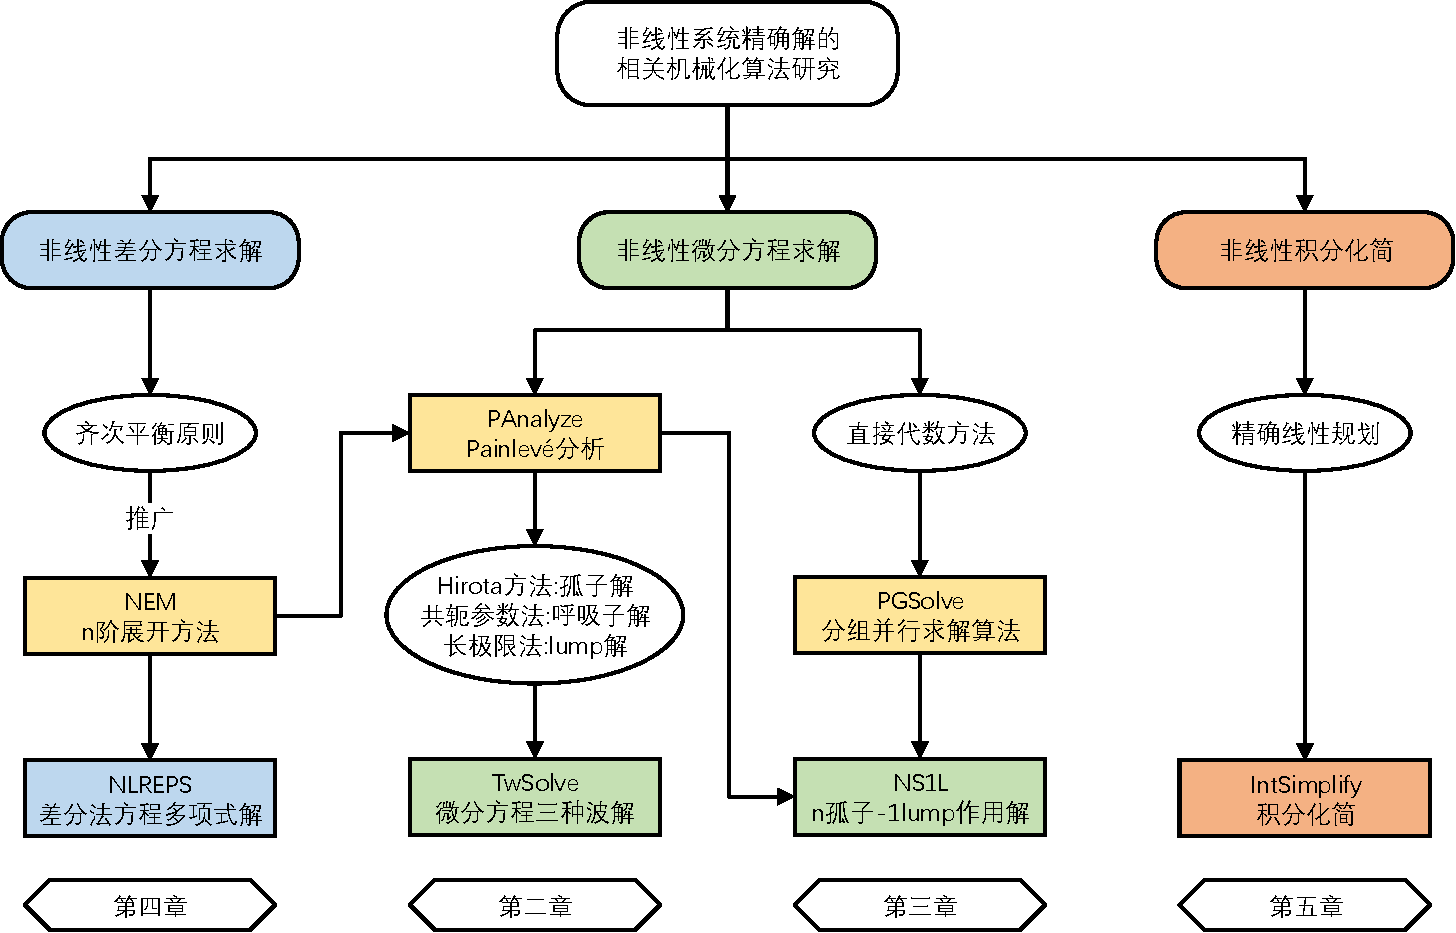
\includegraphics[width=\textwidth]{fig/outline.pdf}
\caption{本文工作大纲图}\label{outline}
\end{figure}

在\refchp{ch02}中, 本文以 \Painleve{} 分析和简单 Hirota 方法为基础, 实现了非线性演化方程三种波解的求解. 其中, 孤子解通过简单 Hirota 方法获得. 获得孤子解之后, 可以通过共轭参数法得到呼吸子解, 通过长极限法得到LUMP解. 本文将上述求解过程打包在TwSolver软件包中.

直接代数方法在微分方程求解中也有广泛的应用, 但其往往伴随着大规模代数方程组的求解. 在第三章中, 本文针对大规模代数方程组求解困难的问题, 设计了一个分组并行求解的算法, 并将其实现为 PGSolve 软件包. 作为PGSolve的应用实例, 本文开发了用直接代数方法求$n$-孤子和1-LUMP相互作用解的软件包 NS1L. 

在第四章中, 受到在微分方程求解中被广泛应用的齐次平衡原则的启发, 本文将其用于求解非线性差分方程的多项式解. 齐次平衡原则通过平衡方程中最高次项的次数来确定解的次数, 只能在一些情况下生效. 本文考虑同时平衡方程中最高$n$项的次数和系数, 提出了$n$阶展开方法来处理齐次平衡原则不能处理的情况, 并将其实现为一个便于拓展应用的软件包 NEM. 基于NEM, 实现了能够求解非线性差分方程所有多项式解的软件包 NLREPS. 

在微分方程的求解中, NEM 能够快速地完善基于齐次平衡原则的求解算法. 在第五章中, 我们以双曲正切方法为例, 基于NEM重新实现了一个NTCM软件包. 该软件包在将双曲正切方法推广到$n+1$维的同时, 利用NEM在阶数分析上的优势, 求解了许多以往不能求解的方程. 同时, 我们也以 \Painleve{} 分析为例展示了 NEM 的作用. 

在第六章中, 因为在非线性微分方程求解的过程中往往需要进行非线性积分表达式的化简, 本文将非线性积分化简作为一个具有挑战性的任务进行研究. 首先, 本文建立了一个代数系统将关于抽象函数的积分多项式视为标准积分项的线性组合. 然后, 基于导数的乘法规则, 设计了一个递归算法来寻找所有的二项合并规则. 最后, 基于这些规则将化简问题转化为一个精确线性规划问题进行求解, 实现了非线性积分表达式化简的软件包 IntSimplify. 

第七章对本文完成的工作进行了总结与讨论,概括了本文的主要研究方法和结论,并提出了对未来工作的展望.
